\section{Messprotokolle}

%Mitschriebe und Lageskizzen
\begin{figure}[!ht]
 \centering
 \includegraphics[width=\textwidth]{fig/Messprotokolle/Mitschrieb1}
 \caption{Mitschrieb 1 vom Versuchstag}
 \label{fig:Mitschrieb_erstes}
\end{figure}

\begin{figure}[!ht]
 \centering
 \includegraphics[width=\textwidth]{fig/Messprotokolle/Mitschrieb2}
 \caption{Mitschrieb 2 vom Versuchstag}
%  \label{fig:}
\end{figure}

\begin{figure}[!ht]
 \centering
 \includegraphics[width=\textwidth]{fig/Messprotokolle/Karte1}
 \caption{Karte vom Versuchstag}
%  \label{fig:}
\end{figure}

\begin{figure}[!ht]
 \centering
 \includegraphics[width=\textwidth]{fig/Messprotokolle/Karte2}
 \caption{Lageskizze der Profile und Kartieung vom Versuchstag}
 \label{fig:Mitschrieb_letztes}
\end{figure}

%Kalibrierung
\begin{figure}[!ht]
 \centering
 \includegraphics[width=0.8\textwidth]{fig/Messprotokolle/Kalibrierung.png}
 \caption{Messprotokoll zur Kalibrierungsmessung}
 \label{fig:MPKalibrierung}
\end{figure}

%Basismessung
\begin{figure}[!ht]
 \centering
 \includegraphics[width=\textwidth]{fig/Messprotokolle/Basismessung}
 \caption{Messprotokoll zur Basismessung}
 \label{fig:MPBasis}
\end{figure}

%Vergleich
\begin{figure}[!ht]
 \centering
 \includegraphics[width=\textwidth]{fig/Messprotokolle/VergleichMagnetometer.png}
 \caption{Messprotokoll zum Vergleich der Protonenmagnetometer und des Fluxgates}
 \label{fig:MPVergleich}
\end{figure}


% Profile
\begin{figure}[!ht]
 \centering
 \includegraphics[width=\textwidth]{fig/Messprotokolle/M21_M2_PM_Seite1}
 \caption{Messprotokoll 1 zu Profil M21-M2, Messgerät Nr. 1}
 \label{fig:MPProfil_erstes}
\end{figure}

\begin{figure}[!ht]
 \centering
 \includegraphics[width=\textwidth]{fig/Messprotokolle/M21_M2_PM_Seite2}
 \caption{Messprotokoll 2 zu Profil M21-M2, Messgerät Nr. 1}
%  \label{fig:}
\end{figure}

\begin{figure}[!ht]
 \centering
 \includegraphics[width=\textwidth]{fig/Messprotokolle/M22_M23_PM_Seite1}
 \caption{Messprotokoll 1 zu Profil M22-M23, Messgerät Nr. 2}
%  \label{fig:}
\end{figure}

\begin{figure}[!ht]
 \centering
 \includegraphics[width=\textwidth]{fig/Messprotokolle/M22_M23_PM_Seite2}
 \caption{Messprotokoll 2 zu Profil M22-M23, Messgerät Nr. 2}
%  \label{fig:}
\end{figure}

\begin{figure}[!ht]
 \centering
 \includegraphics[width=\textwidth]{fig/Messprotokolle/M24_M25_PM_Seite1}
 \caption{Messprotokoll 1 zu Profil M24-M25, neues Messgerät}
%  \label{fig:}
\end{figure}

\begin{figure}[!ht]
 \centering
 \includegraphics[width=\textwidth]{fig/Messprotokolle/M24_M25_PM_Seite2}
 \caption{Messprotokoll 2 zu Profil M24-M25, neues Messgerät}
%  \label{fig:}
\end{figure}

\begin{figure}[!ht]
 \centering
 \includegraphics[width=\textwidth]{fig/Messprotokolle/M26_M27_PM_Seite1}
 \caption{Messprotokoll 1 zu Profil M26-M27, Messgerät Nr. 2}
%  \label{fig:}
\end{figure}

\begin{figure}[!ht]
 \centering
 \includegraphics[width=\textwidth]{fig/Messprotokolle/M26_M27_PM_Seite2}
 \caption{Messprotokoll 2 zu Profil M26-M27, Messgerät Nr. 2}
%  \label{fig:}
\end{figure}

\begin{figure}[!ht]
 \centering
 \includegraphics[width=\textwidth]{fig/Messprotokolle/M28_M29_PM_Seite1}
 \caption{Messprotokoll 1 zu Profil M28-M29, neues Messgerät}
%  \label{fig:}
\end{figure}

\begin{figure}[!ht]
 \centering
 \includegraphics[width=\textwidth]{fig/Messprotokolle/M28_M29_PM_Seite2}
 \caption{Messprotokoll 2 zu Profil M28-M29, neues Messgerät}
%  \label{fig:}
\end{figure}

\begin{figure}[!ht]
 \centering
 \includegraphics[width=\textwidth]{fig/Messprotokolle/M21_M2_Flux_Seite1}
 \caption{Messprotokoll 1 zu Profil M21-M2, Fluxgate}
%  \label{fig:}
\end{figure}

\begin{figure}[!ht]
 \centering
 \includegraphics[width=\textwidth]{fig/Messprotokolle/M21_M2_Flux_Seite2}
 \caption{Messprotokoll 2 zu Profil M21-M2, Fluxgate}
%  \label{fig:}
\end{figure}

\begin{figure}[!ht]
 \centering
 \includegraphics[width=\textwidth]{fig/Messprotokolle/M24_M25_Flux_Seite1}
 \caption{Messprotokoll 1 zu Profil M24-M25, Fluxgate}
%  \label{fig:}
\end{figure}

\begin{figure}[!ht]
 \centering
 \includegraphics[width=\textwidth]{fig/Messprotokolle/M24_M25_Flux_Seite2}
 \caption{Messprotokoll 2 zu Profil M24-M25, Fluxgate}
 \label{fig:MPProfil_letztes}
\end{figure}

%Huette
\begin{figure}[!ht]
 \centering
 \includegraphics[width=\textwidth]{fig/Messprotokolle/EinflussHuette.png}
 \caption{Messprotokoll zum Profil zur Untersuchung der Einflüsse äußerer Störfaktoren auf die Basismessung}
 \label{fig:MPHuette}
\end{figure}


% Wird nicht mehr benötigt:
% \FloatBarrier
% \section{Sonstige Abbildungen} %???Anderer Name
% 
% \begin{figure}[!ht]
%  \centering
%  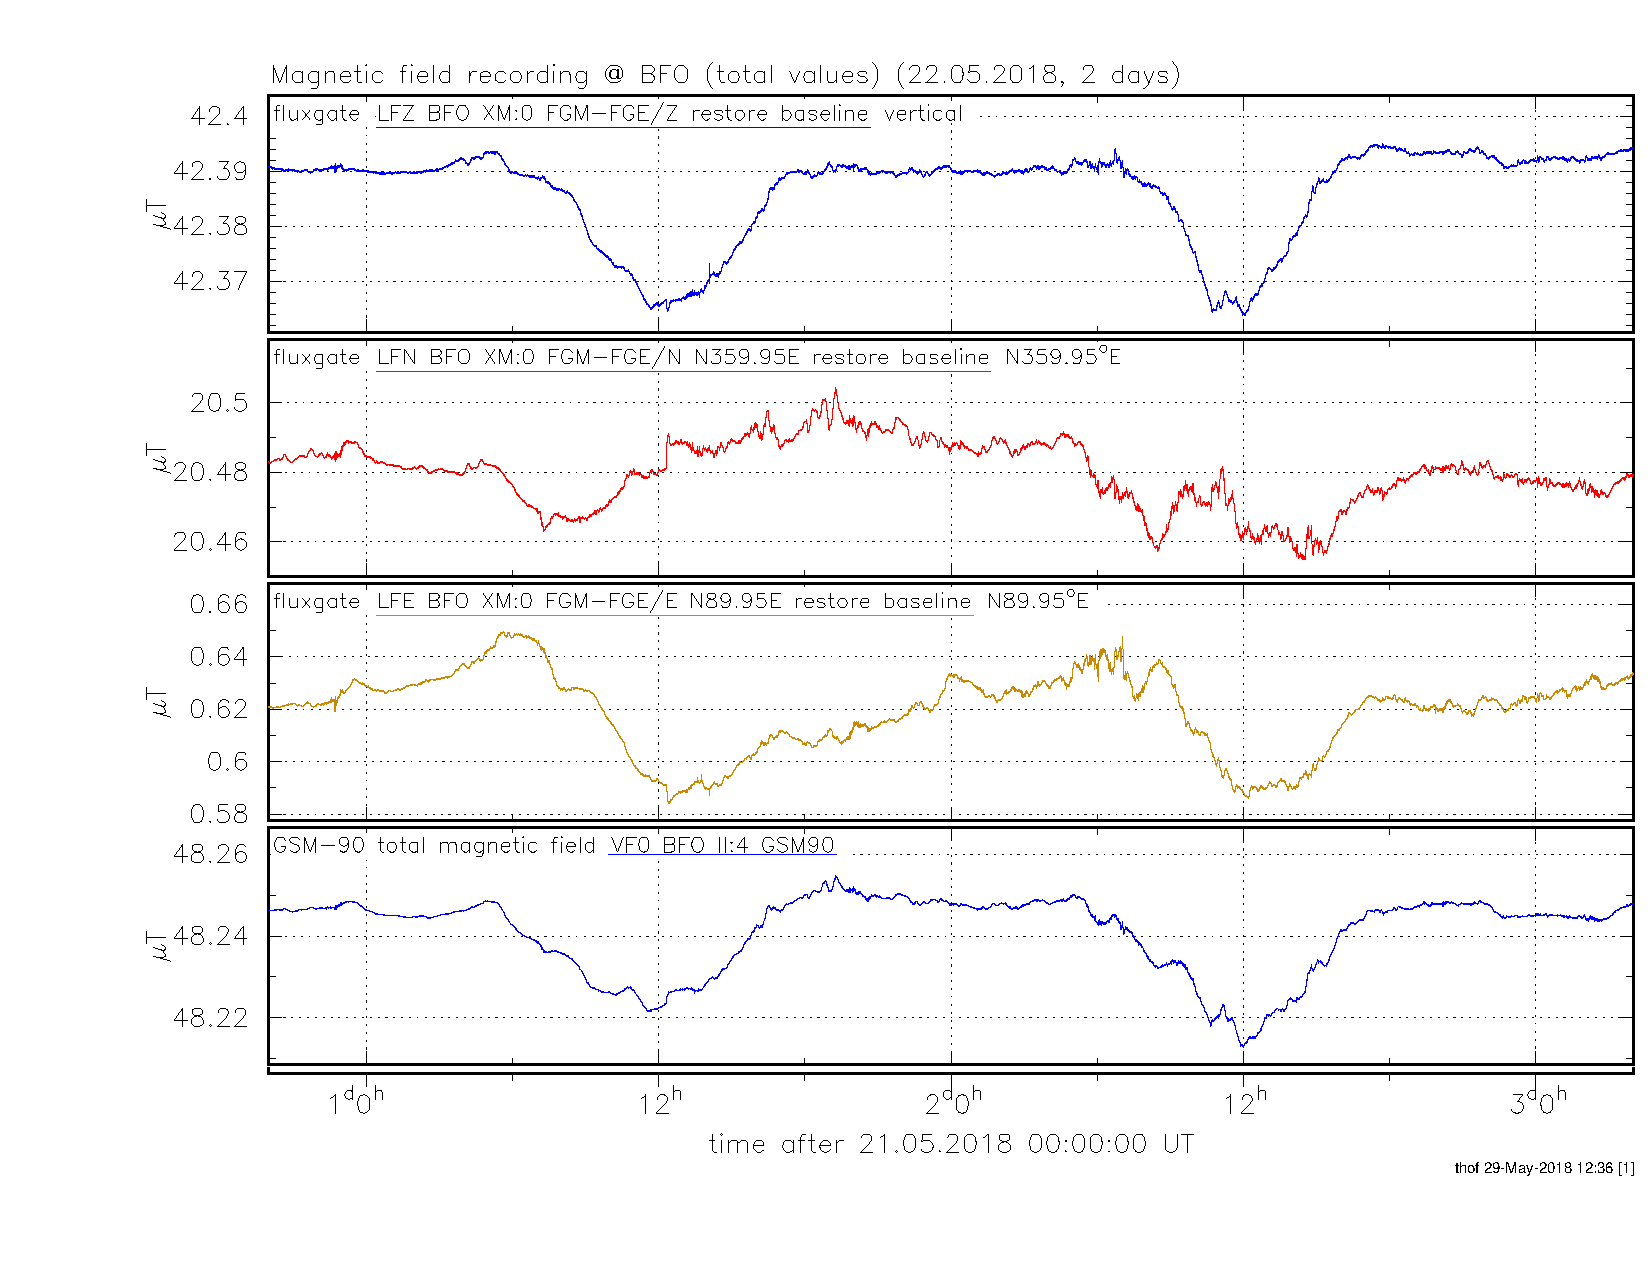
\includegraphics[width=\textwidth]{fig/Magnetfeld_BFO_2_Tage.pdf}
%  \caption[Messung des Magnetfelds am BFO]{Messung des Magnetfelds am BFO. Von oben nach unten: Vertikalkomponente, Nordkomponente und Ostkomponente mit einem Fluxgate gemessen, Totalintensität mit einem Overhauser-Magnetometer gemessen}
%  \label{fig:BFO}
% \end{figure}

% \begin{figure}[!ht]
%  \centering
%  \includegraphics[width=\textwidth]{fig/Messprotokolle/}
%  \caption{}
%  \label{fig:}
% \end{figure}